\section{Kümeleme Metodları} 
\begin{enumerate}
    \item AffinityPropagation
    \item AgglomerativeClustering
    \item Birch
    \item DBSCAN
    \item FeatureAgglomeration
    \item KMeans
    \item MeanShift
    \item MiniBatchKMeans
    \item OPTICS
    \item SpectralClustering
\end{enumerate}

\newpage

\subsection{AffinityPropagation}
Affinity Propagation, özellikle verinin kendi içinde mesajlaşma (iletişim) yeteneğine dayalıdır. Her veri noktasının diğer tüm veri noktalarıyla iletişim kurduğu bir "mesajlaşma" tabanlı bir yaklaşım kullanır. Affinity Propagation, küme merkezlerini otomatik olarak belirler, bu nedenle küme sayısını önceden belirlemeniz gerekmez.

\subsubsection{Çalışma Adımları}
\begin{enumerate}
    \item Veri noktaları arasındaki benzerlikleri ölçmek ve bir benzerlik matrisi oluşturulur. Benzerlik matrisi, her bir veri noktasının diğer tüm veri noktalarına olan benzerlik derecesini içerir.
    \item Her veri noktası, diğer veri noktalarına ne kadar "mesaj göndermeli" ve ne kadar "mesaj almalı" gerektiğini hesaplar. Bu hesaplamalar, iletişim matrisi (responsibility matrix) ve sorumluluk matrisi (availability matrix) olarak adlandırılan iki matris içinde yapılır.
    \item Veri noktaları arasında mesajlaşma sürekli olarak gerçekleşir. Mesajlaşma sonucunda iletişim matrisi ve sorumluluk matrisi güncellenir.
    \item İletişim matrisi ve sorumluluk matrisi kullanarak, her veri noktasının bir küme merkezi olup olmadığını belirler.
    \item Her veri noktasını bir küme merkezine atar ve verileri bu merkezlere göre kümelendirir.
\end{enumerate}

\subsubsection{Hiperparametreler}

\begin{table}[h]
\centering
{\scriptsize\renewcommand{\arraystretch}{0.4}
{\resizebox*{\linewidth}{0.5\textwidth}{
\begin{tabular}{|p{3cm}|p{1cm}|p{1cm}|p{6cm}|}
\hline
Parametre & Type & Default & Açıklama \\ \hline
damping & float & 0.5 & Algoritmanın güncelleme adımlarında kullanılan bir sönümleme faktörüdür. Bu faktör, matris güncellemelerinin istikrarlı hale gelmesine yardımcı olur. Genellikle {[}0.5, 1{]} arasında bir değer alır. \\ \hline
convergence\_iter & int & 15 & Algoritmanın dönüşüm kriterini belirlemek için kullanılır. Belli bir iterasyon sayısına veya sonuçların değişimine dayalı olarak algoritmanın sonlandırılmasını kontrol eder. \\ \hline
preference & array & None & İlk küme merkezi tahminleri üzerinde etkilidir. Özellikle önceden belirlenmiş bir küme sayısı kullanılmadığında, veri noktalarının küme merkezi olma olasılığını ayarlamak için kullanılır. \\ \hline
max\_iter & int & 200 & Maksimum iterasyon sayısı. \\ \hline

\end{tabular}
}}}
\end{table}

\subsubsection{Python Kodu}

\begin{lstlisting}[language=Python, caption=Scikit-learn'de AffinityPropagation örneği.]
import numpy as np

class AffinityPropagation:
    def __init__(self, damping=0.9, max_iter=100, convergence_iter=15):
        # Damping faktoru (0.5 < damping < 1.0)
        self.damping = damping
        # Maksimum iterasyon sayisi
        self.max_iter = max_iter
        # Konsensus iterasyon sayisi
        self.convergence_iter = convergence_iter

    def fit(self, X):
        n_samples = X.shape[0]
        # Baslangicta tercih negativ en kucuk degerlerden olusur
        preference = np.median(X)

        # Sorumluluk (responsibility) matrisi
        R = np.zeros((n_samples, n_samples))
        # Kullanilabilirlik (availability) matrisi
        A = np.zeros((n_samples, n_samples))

        # Benzerlikler guncellenir
        S = X.copy()
        np.fill_diagonal(S, preference)

        for iteration in range(self.max_iter):
            # Sorumluluk guncellemesi
            for i in range(n_samples):
                for k in range(n_samples):
                    max_s = np.max(A[i, :] + S[i, :])
                    R[i, k] = self.damping * R[i, k] + (1 - self.damping) * (S[i, k] - max_s)

            # Kullanilabilirlik guncellemesi
            for i in range(n_samples):
                for k in range(n_samples):
                    if i == k:
                        A[i, k] = self.damping * A[i, k] + (1 - self.damping) * np.sum(np.maximum(R[:, k], 0))
                    else:
                        A[i, k] = self.damping * A[i, k] + (1 - self.damping) * np.minimum(0, R[k, k] + np.sum(np.maximum(R[:, k], 0) - R[i, k]))

            # Konsensus kontrolu
            exemplars = np.where((A + R).diagonal() > 0)[0]

            if len(exemplars) > 0 and iteration >= self.convergence_iter:
                break

        # Kume merkezlerini (exemplar) belirlenir
        cluster_centers_indices = np.where((A + R).diagonal() > 0)[0]

        # Kumeleri atanir
        labels = np.zeros(n_samples)
        for i in range(n_samples):
            labels[i] = np.argmax(S[i, cluster_centers_indices])

        self.cluster_centers_indices_ = cluster_centers_indices
        self.labels_ = labels

    def predict(self, X):
        return self.labels_
\end{lstlisting}

\newpage

\subsection{Agglomerative Clustering}
Agglomerative Clustering, veri noktalarını başlangıçta ayrı ayrı kümelere yerleştirir ve ardından bu kümeleri birleştirerek hiyerarşik bir yapı oluşturur. Etiketlenmemiş verilerle çalışmak için uygundur.

\subsubsection{Çalışma Adımları}
\begin{enumerate}
    \item Başlangıçta, her veri noktası ayrı bir küme olarak kabul edilir. Yani, N veri noktası için N küme oluşturulur.
    \item Belirli bir kriteri (örneğin, mesafe veya benzerlik) kullanarak en yakın iki küme birleştirilir.
    \item Adımlar tekrar edilir ve tüm veri noktaları tek bir büyük küme haline gelene kadar devam eder.
\end{enumerate}

\subsubsection{Python Kodu}

\begin{lstlisting}[language=Python, caption=Scikit-learn'de AgglomerativeClustering.]
import numpy as np

class AgglomerativeClustering:
    def __init__(self, n_clusters=2, linkage="single"):
        # Kume sayisi
        self.n_clusters = n_clusters
        # Linkage -> ['single', 'complete', 'average']
        self.linkage = linkage
        # Etiketler
        self.labels_ = None

    def fit(self, X):
        n_samples = X.shape[0]

        # Her veri noktasi baslangicta ayri bir kume olarak kabul edilir
        clusters = {i: [i] for i in range(n_samples)}

        # Veri noktalari arasindaki mesafe hesaplanir
        distances = np.zeros((n_samples, n_samples))

        for i in range(n_samples):
            for j in range(i + 1, n_samples):
                distances[i, j] = np.sqrt(np.sum((X[i] - X[j]) ** 2))
                distances[j, i] = distances[i, j]

        while len(clusters) > self.n_clusters:
            # Iki kume arasindaki minimum mesafe bulunur
            min_dist = np.inf
            closest_clusters = None

            for c1 in clusters:
                for c2 in clusters:
                    if c1 != c2:
                        if self.linkage == "single":
                            dist = np.min([distances[i, j] for i in clusters[c1] for j in clusters[c2]])
                        elif self.linkage == "complete":
                            dist = np.max([distances[i, j] for i in clusters[c1] for j in clusters[c2]])
                        elif self.linkage == "average":
                            dist = np.mean([distances[i, j] for i in clusters[c1] for j in clusters[c2]])

                        if dist < min_dist:
                            min_dist = dist
                            closest_clusters = (c1, c2)

            c1, c2 = closest_clusters

            # Iki kumeyi birlestir
            clusters[c1].extend(clusters[c2])
            del clusters[c2]

            # Mesafe matrisini guncelle
            new_distances = np.zeros_like(distances)

            for c1 in clusters:
                for c2 in clusters:
                    if c1 != c2:
                        if self.linkage == "single":
                            dist = np.min([distances[i, j] for i in clusters[c1] for j in clusters[c2]])
                        elif self.linkage == "complete":
                            dist = np.max([distances[i, j] for i in clusters[c1] for j in clusters[c2]])
                        elif self.linkage == "average":
                            dist = np.mean([distances[i, j] for i in clusters[c1] for j in clusters[c2]])
                        
                        new_distances[c1, c2] = dist
                        new_distances[c2, c1] = new_distances[c1, c2]

            distances = new_distances

        # Kumeleri etiketle
        labels = np.zeros(n_samples, dtype=int)
    
        for cluster_idx, cluster in enumerate(clusters.values()):
            for sample_idx in cluster:
                labels[sample_idx] = cluster_idx
    
        self.labels_ = labels
\end{lstlisting}

\newpage

\subsection{Birch}
BIRCH (Balanced Iterative Reducing and Clustering Using Hierarchies), veri kümeleme için kullanılan bir hiyerarşik kümeleme algoritmasıdır. BIRCH, büyük veri kümeleri üzerinde etkili bir şekilde çalışabilen bir öğrenme yöntemidir. BIRCH, veriyi kümelemek için özel bir veri yapısı olan bir "CF-Tree" (Clustering Feature Tree) kullanır. İlk olarak, her veri noktası birer "giriş" olarak CF-Tree'ye eklenir. CF-Tree, girişlerin yoğunluğu, merkezi ve varyansı gibi özellikleri temsil eden küçük bir CF (Clustering Feature) vektörü içerir.

\subsubsection{Hiperparametreler}

\begin{table}[h]
\centering
{\scriptsize\renewcommand{\arraystretch}{0.4}
{\resizebox*{\linewidth}{0.4\textwidth}{
\begin{tabular}{|p{3cm}|p{1cm}|p{1cm}|p{6cm}|}
\hline
Parametre & Type & Default & Açıklama \\ \hline
threshold & float & 0.5 & CF-Tree'ye giriş eklerken kullanılan eşik değeridir. Bu değer, her düğümde kaç girişin saklanacağını ve bir düğümün alt düğümlere bölünüp bölünmeyeceğini belirler. Eşik değeri büyüdükçe ağaç daha yüzeysel olur, bu da daha fazla düğümün alt düğümlere bölünmesi anlamına gelir. Bu değeri ayarlayarak kümeleme sonuçları üzerinde büyük bir etkiye sahip olabilirsiniz. \\ \hline
branching\_factor & int & 50 & BIRCH ağacının her düğümünde kaç alt düğümün olacağını belirler. Düğüm sayısını etkiler ve yine ağacın derinliği ve genişliği üzerinde etkilidir. \\ \hline
n\_clusters & int & 3 & Küme sayısını önceden belirlemeniz gereken bir hiperparametredir. \\ \hline

\end{tabular}
}}}
\end{table}

\subsubsection{Python Kodu}

\begin{lstlisting}[language=Python, caption=Scikit-learn'de BIRCH.]
from sklearn.cluster import Birch
from sklearn.datasets import make_blobs
import matplotlib.pyplot as plt

# Veri olusturma
data, _ = make_blobs(n_samples=300, centers=3, cluster_std=1.0, random_state=42)

# BIRCH modeli olusturma
model = Birch(threshold=0.5, n_clusters=3)  # threshold degeri ve kume sayisini belirtin

# Veriyi modele uydurma
labels = model.fit_predict(data)

# Sonuclari gorsellestirme
plt.scatter(data[:, 0], data[:, 1], c=labels, cmap='viridis')
plt.show()
\end{lstlisting}

\newpage

\subsection{DBSCAN}
DBSCAN (Density-Based Spatial Clustering of Applications with Noise), yoğunluğa dayalı bir kümeleme yöntemi olarak çalışır ve noise (gürültü) noktalarını tanıyabilir. Küme sayısını önceden belirlemek gerekmez, bu nedenle veriyi esnek bir şekilde kümeleyebilir. DBSCAN, veri noktalarını üç farklı kategoriye ayırır:
\begin{enumerate}
    \item \textbf{Çekirdek Noktalar (Core Points):} Veri noktası, epsilon yarıçapı içinde en az "MinPts" komşusu varsa bir çekirdek noktasıdır.
    \item \textbf{Sınırlayıcı Noktalar (Border Points):} Veri noktası, epsilon yarıçapı içinde daha az "MinPts" komşusu olmasına rağmen bir çekirdek noktasının içindedir.
    \item \textbf{Gürültü Noktaları (Noise Points):} Veri noktası, epsilon yarıçapı içinde MinPts komşusu olmayan bir noktadır.
\end{enumerate}

Bir çekirdek noktadan başlar ve o noktanın epsilon yarıçapı içindeki tüm noktaları ziyaret eder. Eğer bu noktaların sayısı MinPts'ten büyükse, bir yeni küme başlatılır ve bu noktalar o kümeye atanır. Bu işlem tekrarlanarak tüm çekirdek noktalar ziyaret edilir. Sınırlayıcı noktalar, bir çekirdek noktasının içinde yer alır ve ilgili çekirdek noktanın kümesine atanır. Gürültü noktaları hiçbir kümeyle ilişkilendirilmez ve genellikle kümeleme sonuçlarından çıkarılır.

\subsubsection{Hiperparametreler}

\begin{table}[h]
\centering
{\scriptsize\renewcommand{\arraystretch}{0.4}
{\resizebox*{\linewidth}{0.5\textwidth}{
\begin{tabular}{|p{3cm}|p{1cm}|p{1cm}|p{6cm}|}
\hline
Parametre & Type & Default & Açıklama \\ \hline
eps & float & 0.5 & DBSCAN'da bir veri noktasının komşuluk yarıçapını belirler. Bu parametre, bir veri noktasının epsilon yarıçapı içindeki diğer noktaları incelediği alandır. Doğru epsilon değeri seçmek, kümeleme sonuçlarını etkileyebilir. İyi bir epsilon değeri, verinin yoğunluğuna ve dağılımına bağlıdır. \\ \hline
min\_samples & int & 5 & Bir veri noktasının bir çekirdek nokta olabilmesi için en az kaç komşusu olması gerektiğini belirler. Bu parametre, bir kümenin minimum boyutunu tanımlar. MinPts değerini seçerken, verinin yoğunluğunu dikkate almalısınız. Düşük MinPts değerleri daha fazla küme oluşturabilirken, yüksek MinPts değerleri daha büyük kümeler oluşturur. \\ \hline
n\_clusters & int & 3 & Küme sayısını önceden belirlemeniz gereken bir hiperparametredir. \\ \hline

\end{tabular}
}}}
\end{table}

\newpage

\subsubsection{Python Kodu}

\begin{lstlisting}[language=Python, caption=Scikit-learn'de DBSCAN.]
import numpy as np
from collections import deque

class DBSCAN:
    def __init__(self, eps=0.5, min_samples=5):
        # Komsuluk mesafesi (eps)
        self.eps = eps
        # Minimum komsu sayisi
        self.min_samples = min_samples
        # Etiketler (Gurultu icin -1 alir)
        self.labels = None

    def fit(self, X):
        n_samples = X.shape[0]
        # Baslangicta tum noktalar gurultu olarak kabul edilir (-1)
        self.labels = -np.ones(n_samples)
        cluster_id = 0

        for point_idx in range(n_samples):
            if self.labels[point_idx] != -1:
                continue

            # Komsulari bul
            neighbors = []
            for i in range(X.shape[0]):
                if np.linalg.norm(X[point_idx] - X[i]) <= self.eps:
                    neighbors.append(i)

            # Eger komsu sayisi min_samples'dan az ise, bu nokta gurultudur
            if len(neighbors) < self.min_samples:
                self.labels[point_idx] = -1
            else:
                # Yeni bir kume olustur ve genislet
                self.labels[point_idx] = cluster_id
                queue = deque(neighbors)
        
                while queue:
                    neighbor_idx = queue.popleft()
        
                    if self.labels[neighbor_idx] == -1:
                        # Gurultu noktalarini kumeye ekle
                        self.labels[neighbor_idx] = cluster_id
        
                    if self.labels[neighbor_idx] != -1:
                        continue
        
                    # Bu noktayi kumeye ekle
                    self.labels[neighbor_idx] = cluster_id
        
                    # Bu komsunun komsularini bul
                    new_neighbors  = []
                    for i in range(X.shape[0]):
                        if np.linalg.norm(X[point_idx] - X[i]) <= self.eps:
                            new_neighbors .append(i)
        
                    if len(new_neighbors) >= self.min_samples:
                        queue.extend(new_neighbors)

                cluster_id += 1

    def predict(self, X):
        return self.labels
\end{lstlisting}

\newpage

\subsection{Feature Agglomeration}
Feature Agglomeration, özellik (feature) seviyesinde kümeleme (clustering) yapmak için kullanılan bir kümeleme algoritmasıdır. Bu algoritma, veri setindeki özellikleri benzerliklerine göre gruplandırarak boyut azaltma ve özellik seçimi amaçlar. Feature Agglomeration, özellik benzerlik matrisi (feature similarity matrix) oluşturur. Bu matris, her bir özelliğin diğer özelliklere göre benzerliğini ölçer. Benzerlik matrisi kullanılarak kümeleme algoritması, özellikleri gruplar. Benzer özellikler aynı kümede yer alır.

\subsubsection{Hiperparametreler}

\begin{table}[h]
\centering
{\scriptsize\renewcommand{\arraystretch}{0.4}
{\resizebox*{\linewidth}{0.3\textwidth}{
\begin{tabular}{|p{1cm}|p{2cm}|p{1cm}|p{6cm}|}
\hline
Parametre & Type & Default & Açıklama \\ \hline
n\_clusters & float & 2 & Küme sayısını belirleyen bir hiperparametredir. Kaç küme oluşturulacağını kontrol eder. Küme sayısını belirlerken, verinin doğasını ve amacınızı dikkate almalısınız. \\ \hline
metric & "euclidean", "l1", "l2", "manhattan", "cosine", "precomputed" & None & Benzerlik matrisini hesaplarken kullanılacak benzerlik ölçüsünü belirler. Özellikler arasındaki benzerliği ölçmek için Pearson korelasyonu, kosinüs benzerliği veya başka bir benzerlik metriği seçebilirsiniz. \\ \hline
\end{tabular}
}}}
\end{table}

\newpage

\subsubsection{Python Kodu}

\begin{lstlisting}[language=Python, caption=Scikit-learn'de FeatureAgglomeration örneği.]
import numpy as np

class FeatureAgglomeration:
    def __init__(self, n_clusters=2):
        self.n_clusters = n_clusters
        self.labels_ = None

    def fit(self, X):
        n_features = X.shape[1]

        # Baslangicta her ozellilk bir kume olarak belirlenir
        clusters = {i: [i] for i in range(n_features)}
        self.labels_ = np.arange(n_features)

        # Ozellikler arasindaki mesafe hesaplanir
        distances = np.zeros((n_features, n_features))
        for i in range(n_features):
            for j in range(i + 1, n_features):
                distances[i, j] = np.linalg.norm(X[:, i] - X[:, j])
                distances[j, i] = distances[i, j]

        # Kumeleme islemi
        while len(clusters) > self.n_clusters:
            # Kucuk mesafe bulunur
            min_dist = np.inf
            min_pair = None

            for i in clusters:
                for j in clusters:
                    if i < j:
                        # Iki kume arasindaki ortalama mesafe hesaplanir
                        dist = np.mean([distances[p1, p2] for p1 in clusters[i] for p2 in clusters[i]])
                        if dist < min_dist:
                            min_dist = dist
                            min_pair = (i, j)

            # Kume ciftleri birlestirilir
            i, j = min_pair
            clusters[i].extend(clusters[j])
            del clusters[j]

            # Etiketler guncellenir
            for feature in clusters[i]:
                self.labels_[feature] = i

        return self

    def transform(self, X):
        X_reduced = np.zeros((X.shape[0], self.n_clusters))
        for i in range(self.n_clusters):
            X_reduced[:, i] = np.mean(X[:, self.labels_ == i], axis=1)

        return X_reduced
\end{lstlisting}

\newpage

\subsection{KMeans}
K-Means, veri noktalarını belirli bir sayıda kümeye ayırmak için kullanılır ve her bir kümenin merkezini hesaplar. Küme sayısı kullanıcı tarafından belirlenir.

\subsubsection{Çalışma Adımları}
\begin{itemize}
    \item Başlangıçta, veri noktaları rastgele seçilen "k" küme merkezi ile ilişkilendirilir.
    \item Her veri noktası, öklidyen uzaklık gibi bir yöntemle hesaplanarak en yakın küme merkezine atanır. 
    \item Yeni merkezler, O kümeye ait veri noktalarının ortalaması ile yeni merkezler belirlenir.
    \item Veri noktalarının küme değiştirmemesi ve merkezlerin değişmeyene kadar işlem devam eder.
    \item Son olarak, veri noktaları "k" küme arasında bölünür ve her bir küme kendi merkezine sahip olur.
\end{itemize}

\subsubsection{Hiperparametreler}

\begin{table}[h]
\centering
{\scriptsize\renewcommand{\arraystretch}{0.4}
{\resizebox*{\linewidth}{0.4\textwidth}{
\begin{tabular}{|p{3cm}|p{1cm}|p{1cm}|p{6cm}|}
\hline
Parametre & Type & Default & Açıklama \\ \hline
n\_clusters & int & 8 & K-Means algoritmasıyla oluşturulacak küme sayısını belirler. Bu, kullanıcının belirlemesi gereken bir hiperparametredir. \\ \hline
init & "k-means++", "random" & None & Başlangıç küme merkezlerinin nasıl belirleneceğini kontrol eder. \\ \hline
max\_iter & int & 300 & Atama ve güncelleme adımlarının kaç kez tekrarlanacağını belirler. Algoritmanın konverjansa ulaşana kadar maksimum kaç iterasyon yapacağını kontrol eder. \\ \hline
n\_init & "auto", int & 10 & Başlangıç merkezlerinin farklı başlangıç noktalarıyla çalıştırılacak deneme sayısını belirler. Bu, en iyi sonuçları bulma olasılığını artırır. \\ \hline

\end{tabular}
}}}
\end{table}

\newpage

\subsubsection{Matematik}

$k = 2$ için aşağıdaki belgeleri kmeans ile kümeleyelim.

\begin{table}[h]
    \centering
    {\scriptsize\renewcommand{\arraystretch}{0.3}
    {\resizebox*{\linewidth}{0.3\textwidth}{
    \begin{tabular}{|p{2cm}|p{1cm}|p{1cm}|}
    \hline
    Belge & X & Y \\ \hline
    Belge 1 & 5 & 3 \\ \hline
    Belge 2 & 7 & 5 \\ \hline
    Belge 3 & 6 & 2 \\ \hline
    Belge 4 & 11 & 7 \\ \hline
    Belge 5 & 12 & 9 \\ \hline
    \end{tabular}
    }}}
\end{table}

Başlangıç adımında kümelerin rastgele atanarak:
\begin{itemize}
    \item $K_1$ = Belge 1, Belge 2, Belge 4
    \item $K_2$ = Belge 3, Belge 5, olduğunu varsayalım.
\end{itemize}

Buradan elemanları kullanarak her bir küme için merkezi hesaplayalım. Önce her bir küme içerisindeki X değerleri toplanıp o küme içerisindeki eleman sayısını bölünür. Daha sonra aynı işlem Y değerleri için yapılır.

\begin{itemize}
    \item $K_1 = [\frac{5 + 7 + 11}{3} = 7.67, \frac{3 + 5 + 7}{3} = 5]$
    \item $K_2 = [\frac{6 + 12}{2} = 9, \frac{2 + 9}{2} = 5.5]$, başlangıç için küme merkezlerimiz bunlardır.
\end{itemize}

Şimdi bu işlemleri bir iterasyon boyunca devam ettirerek k-means'i kümelemesini yapalım. Uzaklık hesaplaması için "Euclidean Distance (Öklid Mesafesi)" kullanacağız. Öklid mesafesinin formülü;

\[ \sqrt{(x - M_x)^2 + (y - M_y)^2} \]

Burada:
\begin{itemize}
    \item $x$: Mevcut veri noktasının x değeri.
    \item $y$: Mevcut veri noktasının y değeri.
    \item $M_x$: Küme merkezi noktasının x değeri.
    \item $M_y$: Küme merkezi noktasının y değeri.
\end{itemize}

\newpage

MAX\_ITER = 0 için (Bir nokta için M1 ve M2 mesafelerinden hangisi küçükse nokta o kümeye atanır.);

\begin{figure}[h]
    \centering
    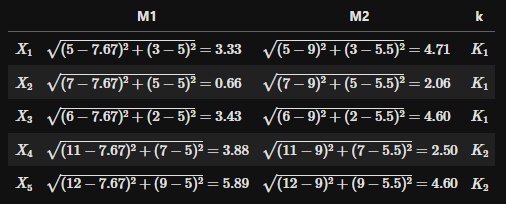
\includegraphics[width=1.0\textwidth]{images/kmeans_step_1.png}
    \caption{MAX\_ITER = 0}
    \label{fig:enter-label}
\end{figure}

Başlangıç adımında $K_1$ kümemiz Belge 1, Belge 2, Belge 4 belgelerinden; $K_2$ kümemiz Belge 3, Belge 5 belgelerinden oluşuyordu. Fakat ilk iterasyondan sonra görünüyorki Belge 3 $K_1$ kümesine, Belge 4 ise $K_2$ kümesine daha yakın. Dolayısıyla yeni kümelerimiz artık;

\begin{itemize}
    \item $K_1$ = Belge 1, Belge 2, Belge 3
    \item $K_2$ = Belge 4, Belge 5 olmuş oldu.
\end{itemize}

Şimdi yeni küme merkezlerimizi hesaplayalım.

\begin{itemize}
    \item $K_1 = [\frac{5 + 7 + 6}{3} = 6, \frac{3 + 5 + 2}{3} = 3.33]$
    \item $K_2 = [\frac{11 + 12}{2} = 11.5, \frac{7 + 9}{2} = 8]$, yeni küme merkezlerimiz bunlardır.
\end{itemize}

\begin{figure}[h]
    \centering
    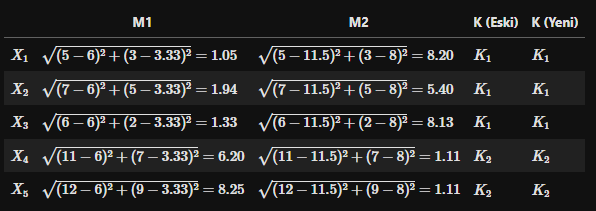
\includegraphics[width=1.0\textwidth]{images/kmeans_step_2.png}
    \caption{MAX\_ITER = 1}
    \label{fig:enter-label}
\end{figure}


Son adımdan da görüneceği gibi K (Eski) ve K (Yeni) sütunları birbirinin aynısı oldu. Yani nihai sonucu elde ettik. Bundan sonra iterasyon yapmamıza gerek yok. 


\subsubsection{Python Kodu}

\begin{lstlisting}[language=Python, caption=Scikit-learn'de KMeans örneği.]
import numpy as np
import pandas as pd
import random

class KMeans:
    def __init__(self, n_clusters=2, max_iter=300):
        # Olusturulacak kume sayisi (k)
        self.n_clusters = n_clusters
        # Maksimum iterasyon sayisi
        self.max_iter = max_iter
        # Kume merkezleri
        self.centroids = None

    def initialize_centroids(self, X):
        # Ilk olarak merkez rastgele secilir.
        centroids = [random.choice(X)]

        # "Euclidean Distance (Oklid mesafesi)" ile diger merkezler uzakliklara gore secilir. (K-Means++)
        for _ in range(1, self.n_clusters):
            # Her bir noktanin mevcut merkezlere olan minimum uzakligi hesaplanir.
            distances = np.min(np.linalg.norm(X - np.array(centroids)[:, np.newaxis], axis=2), axis=0)
            # Olasiliklar normalize edilir.
            distances /= np.sum(distances)

            # Uzaklik olasiliklarina gore yeni merkez secilir.
            next_centroid = X[np.random.choice(len(X), p=distances)]
            centroids.append(next_centroid)

        return np.array(centroids).astype("float32")

    def assign_clusters(self, X):
        # Her nokta en yakin merkeze atanir.
        distances = np.linalg.norm(X[:, np.newaxis] - self.centroids, axis=2).astype("float32")
        return np.argmin(distances, axis=1)

    def update_centroids(self, X, labels):
        # Her kumenin yeni merkezini hesaplanir.
        new_centroids = np.array([X[labels == i].mean(axis=0) if len(X[labels == i]) > 0 else self.centroids[i]
                                    for i in range(self.n_clusters)]).astype("float32")
        return new_centroids

    def fit(self, X):
        # Merkezler baslatilir.
        self.centroids = self.initialize_centroids(X)

        for _ in range(self.max_iter):
            # Her nokta en yakin merkeze atanir.
            labels = self.assign_clusters(X)

            # Yeni merkezler hesaplanir.
            new_centroids = self.update_centroids(X, labels)

            # Merkezler degismediyse islem tamamlanmistir.
            if np.allclose(self.centroids, new_centroids):
                break

            # Merkezler degistiyse yeni merkezler mevcut merkezlerin yerine atanir.
            self.centroids = new_centroids

    def predict(self, X):
        # Her veri noktasi icin en yakin merkezin indeksi alinir.
        labels = self.assign_clusters(X)
        # En yakin merkezin koordinatlari dondurulur.
        labels_coords = np.array([self.centroids[label] for label in labels]).astype("float32")
        return labels_coords, labels
\end{lstlisting}

\newpage

\subsection{MeanShift}
Mean Shift, veri noktalarını veri yoğunluğu temelinde kümelemek için kullanılır. Algoritma, veri noktalarını yoğunluk merkezlerine kaydırarak kümelemeyi gerçekleştirir. Mean Shift, veri yoğunluğuna dayalı olarak doğal kümeleri bulur.

\subsubsection{Çalışma Adımları}
\begin{itemize}
    \item Her veri noktası, başlangıçta kendisinin bir merkez olarak kabul edildiği bir yoğunluk merkezine atanır.
    \item Her bir veri noktası için yoğunluk merkezi hesaplanır. Yoğunluk merkezi, veri noktalarının yoğunluğunun maksimum olduğu noktadır.
    \item Her veri noktası, hesaplanan yoğunluk merkezi pozisyonuna kaydırılır.
    \item 2. ve 3. adımlar tekrar edilir, veri noktaları yoğunluk merkezlerine yaklaştıkça, yoğunluk merkezleri daha da hassaslaşır.
    \item Veri noktaları yoğunluk merkezlerine yaklaşmayı bıraktığında sonlanır. Her bir veri noktası son yoğunluk merkezi ile ilişkilendirilir.
\end{itemize}

\subsubsection{Hiperparametreler}

\begin{table}[h]
\centering
{\scriptsize\renewcommand{\arraystretch}{0.4}
{\resizebox*{\linewidth}{0.3\textwidth}{
\begin{tabular}{|p{3cm}|p{1cm}|p{1cm}|p{6cm}|}
\hline
Parametre & Type & Default & Açıklama \\ \hline
bandwidth & float & None & Bandwidth, yoğunluk merkezlerini hesaplamak için kullanılan pencerenin boyutunu belirler. Büyük bir bant genişliği, daha geniş yoğunluk merkezleri üretebilirken, küçük bir bant genişliği daha küçük ve hassas yoğunluk merkezleri üretebilir. Bandwidth, Mean Shift algoritmasının en önemli hiperparametrelerinden biridir ve doğru bir şekilde ayarlanmalıdır. \\ \hline


\end{tabular}
}}}
\end{table}

\newpage

\subsubsection{Python Kodu}

\begin{lstlisting}[language=Python, caption=Scikit-learn'de MeanShift örneği.]
import numpy as np

class MeanShift:
    def __init__(self, bandwidth=None, max_iter=100, tol=1e-3):
        self.bandwidth = bandwidth
        self.max_iter = max_iter
        self.tol = tol
        self.cluster_centers_ = None
        self.labels_ = None

    def fit(self, X):
        if self.bandwidth is None:
            # Scott kurali
            self.bandwidth = np.mean(np.std(X, axis=0)) * 1.06 * X.shape[0] ** (-1 / 5.)

        # Veri noktalari kopyalanir
        points = np.copy(X)
        for _ in range(self.max_iter):
            new_points = []
            for point in points:
                # Bandwidth icinde olan noktalar bulunur
                in_bandwidth = []
                for x in X:
                    dist = np.sqrt(np.sum((point - x) ** 2))
                    if dist < self.bandwidth:
                        in_bandwidth.append(x)
    
                new_point = np.mean(in_bandwidth, axis=0)
                new_points.append(new_point)

            new_points = np.array(new_points)
            # Degisim miktari
            shift = np.linalg.norm(new_points - points, axis=1)
            if np.all(shift < self.tol):
                break

            points = new_points

        # Kume merkezleri belirlenir
        unique_points = np.unique(np.round(points, decimals=5), axis=0)
        self.cluster_centers_ = unique_points

        # Etiketler
        self.labels_ = np.array([np.argmin([np.sqrt(np.sum((x - center) ** 2)) 
                                 for center in self.cluster_centers_]) for x in X])

    def predict(self, X):
        labels = np.array([np.argmin([np.sqrt(np.sum((x - center) ** 2))
                           for center in self.cluster_centers_]) for x in X])
        return labels
\end{lstlisting}

\newpage

\subsection{MiniBatchKMeans}
MiniBatchKMeans, geleneksel K-Means kümeleme algoritması ile benzer bir yaklaşımı temel alır, ancak büyük veri kümeleri üzerinde daha hızlı çalışmak için bir örnekleme (mini-batch) tabanlı bir yaklaşım kullanır. Bu, büyük veri setlerini hızlı bir şekilde kümelemek için kullanışlıdır.

\subsection{Çalışma Adımları}
\begin{itemize}
    \item MiniBatchKMeans, rastgele seçilen bir alt örneklemi (mini-batch) kullanır.
    \item Mini-batch üzerinde K-Means algoritmasının adımları uygulanır.
    \item Mini-batch'ler sırayla kullanılır ve her bir mini-batch işlendikten sonra küme merkezleri güncellenir.
    \item İterasyonlar belirli bir duruma ulaştığında veya belirli bir iterasyon sayısına ulaştığında algoritma sonlanır.
\end{itemize}

\subsubsection{Hiperparametreler}

\begin{table}[h]
\centering
{\scriptsize\renewcommand{\arraystretch}{0.4}
{\resizebox*{\linewidth}{0.4\textwidth}{
\begin{tabular}{|p{3cm}|p{1cm}|p{1cm}|p{6cm}|}
\hline
Parametre & Type & Default & Açıklama \\ \hline
n\_clusters & int & 8 & Kümelerin sayısını belirler. Bu, kullanıcı tarafından belirlenen bir hiperparametredir. \\ \hline
batch\_size & int & 1024 & Her mini-batch'in boyutunu belirler. Daha büyük bir batch\_size, daha yüksek hesaplama maliyeti demektir. Mini-batch boyutunu seçerken bellek ve hesaplama gücü sınırlamalarını göz önünde bulundurmalısınız. \\ \hline
max\_iter & int & 100 & İterasyonların maksimum sayısını belirler. Algoritmanın ne kadar süre çalışacağını kontrol eder. \\ \hline
init & "k-means++", "random" & "k-means++" & Başlangıç merkezlerini seçme yöntemini belirler. \\ \hline

\end{tabular}
}}}
\end{table}

\newpage

\subsubsection{Python Kodu}

\begin{lstlisting}[language=Python, caption=Scikit-learn'de MiniBatchKMeans.]
import numpy as np

class MiniBatchKMeans:
    def __init__(self, n_clusters=2, batch_size=100, max_iters=100, tol=1e-4):
        self.n_clusters = n_clusters
        self.batch_size = batch_size
        self.max_iters = max_iters
        self.tol = tol
        self.centroids = None

    def fit(self, X):
        n_samples, n_features = X.shape
        # Ilk merkezler rastgele secilir
        random_idx = np.random.choice(n_samples, self.n_clusters, replace=False)
        self.centroids = X[random_idx]

        for i in range(self.max_iters):
            # Mini-batch sec
            minibatch_idx = np.random.choice(n_samples, self.batch_size, replace=False)
            minibatch = X[minibatch_idx]

            # En yakin merkezler bulunur
            distances = np.zeros((minibatch.shape[0], self.n_clusters))
            for i, centroid in enumerate(self.centroids):
                distances[:, i] = np.linalg.norm(minibatch - centroid, axis=1)

            closest_centroids = np.argmin(distances, axis=1)

            # Merkezleri guncelle
            new_centroids = np.copy(self.centroids)
            for c in range(self.n_clusters):
                points_per_centroid = minibatch[closest_centroids == c]
                if points_per_centroid.shape[0] > 0:
                    new_centroids[c] = points_per_centroid.mean(axis=0)

            # Degisim kontrolu
            centroid_shift = np.linalg.norm(self.centroids - new_centroids, axis=None)
            if centroid_shift < self.tol:
                break

            self.centroids = new_centroids

    def predict(self, X):
        distances = np.zeros((X.shape[0], self.n_clusters))
        for i, centroid in enumerate(self.centroids):
            distances[:, i] = np.linalg.norm(X - centroid, axis=1)

        return np.argmin(distances, axis=1)
\end{lstlisting}

\newpage

\subsection{OPTICS}
OPTICS (Ordering Points To Identify the Clustering Structure), yoğunluk temelli kümeleme problemlerinde etkilidir. OPTICS, veri noktalarını sıralayarak kümeleme yapar ve doğal kümeleri ve yoğunluk tabanlı yapısını belirler.

\subsubsection{Hiperparametreler}

\begin{table}[h]
\centering
{\scriptsize\renewcommand{\arraystretch}{0.4}
{\resizebox*{\linewidth}{0.4\textwidth}{
\begin{tabular}{|p{3cm}|p{1cm}|p{1cm}|p{6cm}|}
\hline
Parametre & Type & Default & Açıklama \\ \hline
eps & float & None & Veri noktalarının bir yoğunluk merkezine erişilebilir kabul edilebilecek maksimum uzaklığı belirler. Bu eşik değeri, kümeleme sonuçlarını etkiler. \\ \hline
min\_samples & int & 5 & Bir yoğunluk merkezi olarak kabul edilebilecek minimum veri noktası sayısını belirler. Bu, bir yoğunluk merkezi olarak kabul edilmesi için veri noktalarının çevresinde en az kaç veri noktasının bulunması gerektiğini kontrol eder. \\ \hline

\end{tabular}
}}}
\end{table}

\subsubsection{Python Kodu}

\begin{lstlisting}[language=Python, caption=Scikit-learn'de OPTICS örneği.]
from sklearn.cluster import OPTICS
from sklearn.datasets import make_blobs
import matplotlib.pyplot as plt

# Veri olusturma
data, _ = make_blobs(n_samples=300, centers=4, cluster_std=1.0, random_state=42)

# OPTICS modeli olusturma
model = OPTICS()  # Hiperparametreler belirtilmezse varsayilan degerler kullanilir.

# Veriyi modele uydurma
model.fit(data)

# Sonuclari gorsellestirme
plt.scatter(data[:, 0], data[:, 1], c=model.labels_, cmap='viridis')
plt.show()
\end{lstlisting}

\newpage

\subsection{SpectralClustering}
Spectral Clustering, veri noktalarının benzerlik grafiği üzerinden kümeleme yapma yeteneğine sahiptir. Bu algoritma, veri noktalarının benzerlik matrisini kullanarak bir graf oluşturur ve bu grafiği kullanarak veri kümelemesi yapar.

\subsubsection{Çalışma Adımları}
\begin{itemize}
    \item Veri noktaları arasındaki benzerliği ölçen benzerlik matrisi oluşturulur. Benzerlik matrisi, bir grafı temsil eder. Her bir veri noktası bir düğüm ve benzerlikler arasındaki değerler ise kenarlar olarak düşünülür.
    \item Graf üzerinde Laplace matrisi hesaplanır. Laplace matrisi, grafın yapısını ve veri noktalarının bağlantılarını yakalar.
    \item Laplace matrisinin özdeğer ayrışımı (eigendecomposition) yapılır ve özdeğerler kullanılarak veri noktaları spektral uzayda temsil edilir.
    \item Elde edilen spektral uzayda k-means veya diğer kümeleme yöntemleri kullanılarak veri noktaları kümelere ayrılır.
\end{itemize}

\subsubsection{Hiperparametreler}

\begin{table}[h]
\centering
{\scriptsize\renewcommand{\arraystretch}{0.4}
{\resizebox*{\linewidth}{0.4\textwidth}{
\begin{tabular}{|p{3cm}|p{1cm}|p{1cm}|p{6cm}|}
\hline
Parametre & Type & Default & Açıklama \\ \hline
n\_clusters & int & 8 & Küme sayısını belirler. Hangi sayıyı seçeceğinizi veri yapısına ve analiz amacınıza bağlı olarak belirlemelisiniz. \\ \hline
affinity & str & "rbf" & Benzerlik matrisi hesaplama yöntemini belirler. Öklidyen uzaklık veya kosinüs benzerliği gibi farklı metrikler kullanılabilir. \\ \hline
n\_neighbors & int & 10 & Grafiği oluştururken her veri noktasının en yakın kaç komşusunu kullanacağınızı belirler. Bu, grafın yoğunluğunu ve bağlantılarını etkiler. \\ \hline
eigen\_solver & "arpack", "lobpcg", "amg" & "k-means++" & Özdeğer ayrışımını yaparken kullanılacak algoritmayı belirler. \\ \hline
\end{tabular}
}}}
\end{table}

\newpage

\subsubsection{Python Kodu}

\begin{lstlisting}[language=Python, caption=Scikit-learn'de SpectralClustering örneği.]
import numpy as np
from sklearn.cluster import KMeans
from scipy.spatial.distance import cdist
from sklearn.preprocessing import normalize

class SpectralClustering:
    def __init__(self, n_clusters=2, sigma=1.0):
        # Kume sayisi
        self.n_clusters = n_clusters
        # Sigma
        self.sigma = sigma

    def fit(self, X):
        # Agirlik matrisi olusturulur
        pairwise_sq_dists = cdist(X, X, "sqeuclidean")
        W = np.exp(-pairwise_sq_dists / (2 * self.sigma ** 2))
        np.fill_diagonal(W, 0)


        # Derece matrisi olusturulur
        D = np.diag(np.sum(W, axis=1))

        # Laplace matrisi olusturulur
        L = D - W

        # Laplace matrisnin ozdeger ve ozvektorleri hesaplanir
        eigenvalues, eigenvectors = np.linalg.eigh(L)

        # En kucuk n_clusters ozdegere karsilik gelen ozvektorler secilir
        idx = np.argsort(eigenvalues)[:self.n_clusters]
        H = eigenvectors[:, idx]

        # Secilen ozvektorler normallestirilir
        H_normalized = normalize(H, norm="l2", axis=1)

        # KMeans ile kumeler belirlenir
        kmeans = KMeans(n_clusters=self.n_clusters)
        self.labels_ = kmeans.fit_predict(H)
        return self

    def predict(self, X):
        return self.labels_
\end{lstlisting}

\newpage